\documentclass[leqno]{article}
\usepackage[utf8]{inputenc}
\usepackage[T1]{fontenc}
\author{Colin Roberts}
\title{Math 676 (Olivier) Class Notes}
\usepackage[left=3cm,right=3cm,top=3cm,bottom=3cm]{geometry}
\usepackage{amssymb, amsmath ,cleveref ,thmtools, amsthm, mathtools}
\usepackage{enumerate}
\usepackage{hyperref}
\usepackage{color}

%%fonts
%??


\makeatletter
\def\thmhead@plain#1#2#3{%
  \thmname{#1}\thmnumber{\@ifnotempty{#1}{ }\@upn{#2}}%
  \thmnote{ {\the\thm@notefont#3}}}
\let\thmhead\thmhead@plain
\makeatother
\theoremstyle{definition}
\newtheorem{definition}{Definition}[section]
\newtheorem*{remark}{Remark}
\newtheorem*{example}{Example}
\newtheorem*{question}{Question}
\newtheorem*{exercise}{Exercise}

\theoremstyle{remark}
\newtheorem*{solution}{Solution}

\theoremstyle{theorem}
\newtheorem{theorem}{Theorem}[section]
\newtheorem{corollary}{Corollary}
\newtheorem{proposition}{Proposition}
\newtheorem{axiom}{Axiom}

\newcommand{\R}{\mathbb{R}}
\newcommand{\Q}{\mathbb{Q}}
\newcommand{\F}{\mathbb{F}}
\newcommand{\A}{\mathcal{A}}
\newcommand{\N}{\mathbb{N}}
\newcommand{\im}{\mathrm{Im}}
\newcommand{\re}{\mathrm{Re}}

\begin{document}
\maketitle
\tableofcontents
\pagebreak

\section{Physics Prerequisites}	
\subsection{Waves}  

We describe the electromagnetic field via $(\vec{E}(t,x), \vec{B}(t,x))$ with $\vec{E}$ representing the electric field and $\vec{B}$ representing the magnetic field.  Of course, $t$ represents time and $x$ represents position ($x$ could potentially be a vector in $\R^3$).

\begin{itemize}
\item Suppose we have a wave that is described by a scalar field $\phi(t,x)$, which is a solution to the wave equation
\[
\partial_t^2 \phi - c^2 \Delta \phi = 0.
\]
Then we say the intensity is $I(t,x)=|\phi(t,x)|^2$. We denote $\phi(0,x)$ by $\phi_0 (x)$. 
\item Equivalently, we could choose to represent this solution in Fourier space by transforming from spatial coordinates $x$ to wave vector coordinates $k$.  We then have
\[
\phi(t,x)=\frac{1}{(2\pi)^{3/2}} \int_{\R^3} \hat{\phi}_0 (k) e^{i(kx-\omega t)} dx.
\]
By Fourier-Plancherel we then have that 
\[
\int_{\R^3} |\phi(t,x)|^2 dx = \int_{\R^3} |\hat{\phi}_0 (k)|^2 dk.
\]
It then follows that in Fourier space, we have 
\[
-\omega^2 +c^2 |k|^2=0
\]
iff $\phi$ is a solution to the wave equation. In other words, $\phi$ satisfies the \emph{dispersion relation} $\omega^2 = c^2 |k|^2$.

\item $\hat{\phi}_0(k)$ is smooth and has compact support.  Meaning that $\hat{\phi}_0(k)=0$ for $|k|\geq K$ for some positive $K$.  

\item We see that $\phi(t,x)$ has the following form:
\begin{center}
\begin{figure}[h]
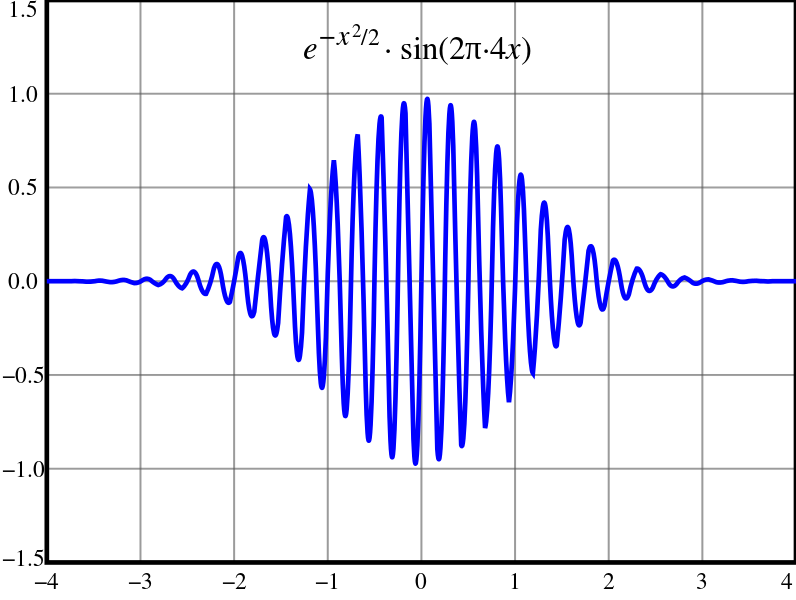
\includegraphics[width=6cm]{wavepacket.png}
\end{figure}  
\end{center}

\item Finally we have that $\hat{\phi}(t,k)=\hat{\phi}_0 (k)e^{i(kx-\omega t)}$ as the time-evolved state.

\end{itemize}

\subsection{Position and Momentum Operators}

We will use the following notation for the inner product $(u,v)=\int_{\R^3} \overline{u}(x)v(x)dx$ and for the norm $\|u\|^2=(u,u)$.

\begin{definition}
The \emph{average position of a wave packet} is 
\[
\langle x(t) \rangle \coloneqq \frac{\int_{\R^3}x |\phi(t,x)|^2 dx}{\|\phi(t,\cdot)\|^2}.
\]
The \emph{momentum} is then $\vec{p}=\hbar \vec{k}$.  Then the \emph{average value of the momentum for the wave packet} is given by
\[
\langle p(t) \rangle \coloneqq \frac{\int_{\R^3} \hbar k |\hat{\phi}(t,k)|^2 dk}{\|\hat{\phi}(t,\cdot)\|^2}.  
\]
From here on out we restrict to normalized states, i.e., $\|\phi(t,\cdot)\|=1$.
\end{definition}

\begin{definition}
The \emph{position operator} $X_i \varphi = x_i \varphi$ for $i=1,2,3$.  Note that for $\phi \in L^2(\R^3)$ we may not have that $X_i \colon L^2(\R^3) \to L^2(\R^3)$. 
\end{definition}

\begin{definition}
The momentum operator is $P_j \varphi(x) = i\hbar \frac{\partial}{\partial x_j} \varphi(x)$ for $j=1,2,3$. 
\end{definition}

\begin{remark}
Of course we can Fourier transform the above operators.  The Fourier transform of the position operator becomes differentiation with respect to $k$ and the Fourier transform of the momentum operator becomes multiplication by $\hbar k$.  
\end{remark}

It follows that we can write the expected values for the position and momentum in the following way:
\begin{align*}
\langle X_j \rangle &= (X_j \phi(t,\cdot),\phi(t,\cdot)),\\
\langle P_j \rangle &= (P_j \phi(t,\cdot),\phi(t,\cdot)).
\end{align*}

\begin{proposition}
$X_j$ and $P_j$ are symmetric operators.  Meaning that for smooth functions $\phi,\psi$ we have that
\begin{align*}
(X_j \phi,\psi) &= (\phi, X_j \psi),\\
(P_j \phi,\psi) &= (\phi, P_j,\psi).
\end{align*}
Moreover, $X_j$ and $P_j$ satisfy the Heisenberg commutation relations:
\begin{align*}
X_i P_j &= P_j X_i,  && i\neq j\\
P_iX_i - X_i P_i &= -i\hbar \mathbf{I}.
\end{align*}
\end{proposition}

\begin{proof}
Left as an exercise. \emph{Hint: $P_i(X_i \varphi)-X_i(P_i\varphi)=-i\hbar \varphi$.}
\end{proof}

Since we were able to find the center of the wave packet, $\langle X_i \rangle$ (for position, at least).  We wish to find the width of the wave packet in order to fully characterize the state.  We have that the width is
\begin{align*}
(\Delta X_j)^2 &= \int_{\R^3} |x_j - \langle X_j \rangle |^2 |\phi(t,x)|^2 dx\\
&= \|x_j \phi(t,\cdot \|^2 - (\langle X_j \rangle)^2.
\end{align*}

\begin{proposition}
Let $A, B$ be symmetric operators that satisfy Heisenberg's commutation relation $AB-BA=i\hbar \mathbf{I}$, then
\[
\|A\varphi\|^2 \|B\varphi\|^2 \geq \frac{\hbar^2}{4} \|\varphi\|^4.
\]
\end{proposition}

\begin{proof}
Let $\lambda \in \R$. So then $\|(A+i\lambda B)\varphi)\|^2=\|A\varphi\|^2 +2\mathrm{Re}(A\varphi,i\lambda B \varphi)+\lambda^2 \|B\varphi\|^2$. Now we have
\begin{align*}
\mathrm{Re}(A\varphi,i\lambda B\varphi) &= -\lambda \im (A\varphi,B\varphi)\\
&= -\lambda \im (\varphi, AB\varphi) && \textrm{since $A,B$ is symmetric}\\
&= -\lambda \im (BA\varphi,\varphi)\\
&= -\lambda \im \int_{\R^3} \overline{BA\varphi}\varphi dx \\
&= \lambda \im \int_{\R^3} \overline{\varphi}BA\varphi dx.
\end{align*}
So now, 
\begin{align*}
2\re (A\varphi,i\lambda B \varphi)&= -\lambda \im (\varphi,(AB-BA)\varphi)\\
&= -\lambda \im (i\hbar \|varphi\|^2)\\
&= -\lambda \hbar \|\varphi\|^2.
\end{align*}
So,
\begin{align*}
\|A\varphi\|^2-\lambda \hbar \|\varphi\|^2 - \lambda^2 \|B\varphi\|^2 &\geq 0 && \forall \lambda \in \R\\
\implies \hbar^2 \|\varphi\|^4 &\leq 4 \|B\varphi\|^2\|A\varphi\|^2 && \textrm{using a discrimant or something}\\
\implies \|B\varphi\|\|A\varphi\|^2 &\geq \frac{\hbar}{2}\|\varphi\|^2.
\end{align*}
\end{proof}

\begin{theorem}
Define $\Delta X_i = \sqrt{\|X_i\phi\|^2-\langle X_i \rangle^2}$, $\Delta P_i = \sqrt{\|P_i \hat{\phi}\|^2 - \langle P_i \rangle^2}$.  Then $\Delta X_i \Delta P_i \geq \frac{\hbar}{2}$ when $\|\phi\|=1$.  
\end{theorem}

\begin{proof}
We define $\tilde{X}_i = X_i - \langle X_i \rangle \mathbf{I}$ and $\tilde{P}_i = P_i - \langle P_i \rangle \mathbf{I}$.  \\
Claim: $\tilde{X}_i$ and $\tilde{P}_i$ satisfy Heisenberg's commutation relation.  Then apply the above proposition and we are done.
\end{proof}

\subsection{Wave Packets in 1D}

Now we wish to investigate the wave packets a bit more to find out specific characteristics.  We have
\[
\phi(t,x)=\frac{1}{(2\pi)^{3/2}} \int_\R \hat{\phi}_0 (k) e^{i(kx-\omega t)} dk,
\]
with  $\hat{\phi}_0 (k)=0$ for $k\leq 0$.  \\
\textbf{Goal:} Characterize $\langle X \rangle = (X\phi,\phi)$ with $\|\phi\|=1$ and $\langle P \rangle$ when $\phi$ satisfies the wave equation.  We can factor the wave equation into 
\[
(\partial_t -c\partial_x)(\partial_t+c\partial_x)\phi=0.
\]
We write the general solution $\phi=\phi_+ + \phi_-$ which correspond to waves traveling forward (backward) denoted with + (-). So now we have
\begin{align*}
\frac{d}{dt} \langle X \rangle &= (X \partial_t \phi,\phi)+(X\phi,\partial_t \phi)\\
&= -2 \re (X\phi,\partial_t \phi)\\
&= -2 \re (X\phi, C\partial_x \phi)\\
&= -2c \re \int_\R x\overline{\phi} \partial_x \phi dx\\
&= -c \int_\R x \partial_x |\phi|^2 dx &&\textrm{by integrating by parts, of course}\\
&= c \int_\R |\phi|^2dx = c.
\end{align*}
This means that $\frac{d}{dt}\langle X \rangle =c$. This makes physical sense, since of course a wave should propagate at the speed of light.

Next, we have $\langle P \rangle = \int_\R \hbar k |\hat{\phi}(t,k)|^2dk$.  Then $\phi(t,x)=\frac{1}{(2\pi)^{1/2}}\int_\R \hat{\phi}_0 (k)e^{i(kx-\omega t)} dx$. So $\hat{\phi}(t,k)=\hat{\phi}_0(k)e^{-i\omega t}$.  Then $|\hat{\phi}(t,k)|^2=|\hat{\phi}(k)|^2$ which implies that $\frac{d}{dt}\langle P \rangle =0$.  Physically this is saying that the expected value of the momentum should remain constant, which fits with our classical understanding.

\subsection{Dispersive Propagation}

Suppose that we have $\omega = \omega(k)$.  Then
\begin{align*}
\langle X \langle = (X\phi,\phi) = (X\hat{\phi},\hat{\phi}),
\end{align*}
and
\begin{align*}
\hat{X\phi}(k)=i\nabla_k \hat{\phi}.
\end{align*}
So, $\hat{\phi}(t,k)=\hat{\phi}_0(k)e^{-i\omega(k)t}$ and we have
\begin{align*}
\nabla_k \hat{\phi}(t,k)&= \nabla_k \hat{\phi}_0 (k)e^{-i\omega(k)t}-i\nabla_k \omega(k)\hat{\phi}_0(k)e^{-i\omega(k)t}\\
\implies \nabla_k \hat{\phi}\overline{\hat{\phi}}&=\nabla_k \hat{\phi}_0 \overline{\hat{\phi}}_0 - i\nabla_k \omega(k) |\hat{\phi}_0 (k)|^2\\
\implies \frac{d}{dt} \langle X \rangle &=\int_{\R^3} \nabla_k \omega(k)|\hat{\phi}_0 (k)|^2 dk\\
&= \langle \nabla_k \omega(k) \rangle.
\end{align*}
Note that $\nabla_k \omega(k)=V_g (k)$ is known as the \emph{group velocity}.

So when we have $\omega(k)=ck$ from the wave equation, then we have $\nabla_k \omega(k)=c$ which means there is no dispersion of our wave.  As before, we have $\frac{d}{dt} \langle P \rangle = 0$.

With the Sch{\"o}dinger equation, we expect to have the wave disperse.  Meaning that the wave packet will widen as time passes.  We have $\Delta X_i^2=\|X_i \phi \|^2 - (\langle X_i \rangle)^2$. Then we claim that $\Delta X_i^2=At^2+at+b$.  

\begin{exercise}
Show that $A=\int_{\R^3} |\nabla_k \omega|^2|\hat{\phi}_0(k)|^2-\langle V_g \rangle ^2$.
\end{exercise}

From the De Broglie relation we have $E=\frac{\hbar^2 |\vec{k}|^2}{2m}=\hbar \omega$ which implies that $\omega(k)=\frac{\hbar|\vec{k}|^2}{2m}$.  So we can find that the expression for the wave packet follows from below.
\begin{align*}
\phi(t,x)&=\frac{1}{(2\pi)^{3/2}} \int_{\R^3} \hat{\phi}_0 (k) e^{i\left(k\cdot x - \frac{\hbar |\vec{k}|}{2m}t\right)}dk\\
i\hbar \partial_t \phi &= \frac{\hbar^2}{2m}\int_{\R^3}|k|^2 \hat{\phi}_0 (k) e^{i0}dk\\
&= \frac{-\hbar^2}{2m}\Delta \phi.
\end{align*}
This implies the \emph{free Sch{\"o}dinger equation} $i\hbar \partial_t \phi = \frac{-\hbar^2}{2m}\Delta \phi$.





\pagebreak
\section{References}
\begin{enumerate}[1.]
\item Reed Simon
\end{enumerate}

\end{document}